\documentclass{article}[11pt]
%
% 
%
%-------------------------------------------------------------------
\parindent 0pt
\parskip 0.75ex
\renewcommand{\baselinestretch}{1.03}
\renewcommand{\topfraction}{0.9}
\renewcommand{\textfraction}{0.01}
\renewcommand{\floatpagefraction}{0.99} 
\addtolength{\textwidth}{6mm}
\addtolength{\textheight}{1cm}
\usepackage{graphicx}
\usepackage{hyperref}
\usepackage{wrapfig}
\usepackage{color}
\usepackage{pifont}


\newcommand{\pointout}[1]{
\vskip 3mm
\begin{minipage}[c]{\linewidth}
\hrule
\vskip 2mm
\begin{minipage}[c]{0.1\linewidth}
{\Huge\color{red}\ding{43}}
\end{minipage}
\begin{minipage}[c]{0.9\linewidth}
#1
\end{minipage}
\vskip 2mm
\hrule
\end{minipage}
\vskip 3mm
}

\newcommand{\warning}[1]{
\vskip 3mm
\begin{minipage}[c]{\linewidth}
\hrule
\vskip 2mm
\begin{minipage}[c]{0.1\linewidth}
{\Huge\color{red}{\fontencoding{U}\fontfamily{futs}\selectfont\char 66\relax}}
\end{minipage}
\begin{minipage}[c]{0.9\linewidth}
#1
\end{minipage}
\vskip 2mm
\hrule
\end{minipage}
\vskip 3mm
}




\makeatletter
\def\verbatim{\footnotesize\@verbatim \frenchspacing\@vobeyspaces \@xverbatim}
\makeatother

\definecolor{darkred}{rgb}{0.6,0.2,0}


\begin{document}



\title{RCDAQ, a lightweight yet powerful data acquisition system}
\author{Martin L. Purschke}
\maketitle

\tableofcontents

\newpage

\section{Changelog}

\subsection{February 20, 2020}
\begin{itemize}
\item I added a command \verb|daq_get_lastfilename| (see
  chapter~\ref{CommandOverview}) that returns the most recent (or
  current) filename, if any. If you took a run without logging, the
  name will be empty. The purpose of this command is for automated,
  scripted measurements. You can obtain the last filename \emph{after}
  the run has ended, so you can use it to start some analysis on the
  file right away after the run ends. Before it was hard to get at
  that filename in a script.

\end{itemize}

\subsection{February 13, 2019}
\begin{itemize}
\item I added a new built-in pseudo device \verb|device_gauss|.  Its
  only role is to provide data to monitor for the tutorial of the
  companion ``pmonitor'' manual. I provide a
  \verb|setup_pmonitor_tutorial.sh| script that sets all up properly if you want
  to run all parts of the tutorial.
\end{itemize}


\subsection{March 13, 2018}
\begin{itemize}
\item I added a new built-in pseudo device \verb|device_rtclock|.  It
  allows you to measure the event timing, and the distance in time to
  the most recent event. See chaper~\ref{eventtiming}
\end{itemize}

\subsection{February 22, 2017}
\begin{itemize}
\item I added the concept of a named RCDAQ instance. We found that we
  are often running multiple RCDAQ systems (such as the main DAQ and
  the wirechamber readout at Fermilab). This has sometimes led to
  confusion which instance you are interacting with. The name
  defaults to the hostname, and can be set with
  \verb|rcdaq_client daq_setname|, and retrieved with
  \verb|rcdaq_client daq_getname|.  The aliases have also been
  updated to make the command shortcuts, and the GUIs show the name
  now, too. 
\item The \verb|daq_status| used to show ``logging enabled'', and nothing if
  disabled. So the absence of the ``enabled'' message indicated
  that we are not logging. That has led to a number of operator
  errors. \verb|daq_status| now shows ``enabled'' or ``disabled''. 
\item I have added the start of the web service on the standard port
  8899 in the template setup script ``\verb|setup.sh|''. If this port
  is taken on your system, you need to change it. 

\end{itemize}

\subsection{August 30, 2016}
\begin{itemize}
\item Added documentation about the newly implemented web-based controls. 
\end{itemize}

\subsection{February 28, 2016}
\begin{itemize}
\item expanded the chapter~\ref{installation} with many more details
  and step-by-step instructions
\item  added a chapter about the PSI DRS4 evaluation board 
\end{itemize}

\subsection{August 27, 2015}
\begin{itemize}
\item  added two new devices device\_file\_delete and device\_filenumbers\_delete, which
  delete the file after it has been read. See page~\pageref{delete} for a description and application.
\end{itemize}

\subsection{August 15, 2015}
\begin{itemize}
\item the rcdaq\_server process now defines a number of environmental
  variables, principally for the benefit of  device\_command. The
  resulting process, usually a script, can use the variables to obtain important
  information it might need. See page~\pageref{environment}.
\end{itemize}

\newpage

\section{Introduction}


\subsection{What This is About}

RCDAQ is a data acquisition package which is used in the R\&D efforts
of the PHENIX and sPHENIX experiments at the Relativistic Heavy Ion
Collider.  The experiment has its main data acquisition which fills a
room about size of a squash court. For a variety of R\&D efforts, it
was necessary to get a smaller, portable, and lightweight data
acquisition system which would support test beams, electronics
developments, cosmic ray tests, and the like.

Meanwhile, the system is in use for a number of other projects, such
as a number of PET scanners for medical imaging applications, the
readout of a GEM detector, and for tests and the characterization of
Silicon Photomultipliers.


The development of RCDAQ was governed by a number of design principles:

\begin{description}

\item {\bf format-compatible with the main PHENIX data acquisition
  system.} In this way, the readout of a new device needs to get
  implemented and debugged only once, and is ready to go once the new
  component is integrated in the main DAQ system. This also allows to
  reuse most tools, such as online monitoring components, during the
  running of the main experiment.

\item {\bf compatible with the PHENIX online monitoring and analysis
  framework.}  This allows to reuse the code developed during the R\&D
  phase and test beams once the new detector or component is installed
  in PHENIX. The online monitoring of several new detectors has its
  roots in the online monitoring used and refined in a test beam.

\item {\bf lightweight and able to run on most modern Linux distributions.}
  You do not have to devote your system to the task of running the
  DAQ. (As a rule of thumb, if your system has a working version of the 
  root package, you will be able to install RCDAQ and the assorted
  components). RCDAQ is also able to build and run on a Raspberry Pi.

\item {\bf powerful and fast.} The most demanding device supported by
  RCDAQ produces sustained data rates of 400\,MB/s.

\item {\bf client-server based.} This will allow you to work in a
  network-transparent way, for example, control the main DAQ running on
  a powerful server natively from your desktop or laptop.

\item {\bf based on a plugin concept.} In order to make the package
  adaptable to a large number of tasks, most of the actual readout
  capabilities and support for the readout of particular devices is
  added through plugins. In this way, we are able to make the core
  package available outside the PHENIX collaboration because no
  proprietary or commercial libraries or drivers (which are needed for
  some PHENIX hardware) need to be distributed.

\item {\bf extensive support for automated, scripted acquisitions.}

\item {\bf no configuration \emph{files}}. By definition,
  configuration files require you to learn their syntax. In most
  cases, configuration file formats, say, XML, do not support loops,
  conditions, formal parameters, or error handling, which is why most
  systems have moved away from the much-hyped XML format. We already
  have the best parser for configuration input -- the Unix shell. It
  fulfills all of the above requirements (loops, conditions, parameters,
  and error handling). Each interaction with RCDAQ is a Unix shell
  command. In this way, there are no configuration files, but
  configuration \emph{scripts} which you execute to configure your
  system.

\item {\bf Elog Support}. RCDAQ natively supports the \emph{elog}
  electronic logbook, developed and maintained by Stefan Ritt at the
  Paul-Scherrer Institute in Switzerland. RCDAQ can be configured to
  make automated elog entries to help you keep track of the data you
  acquire.  You can add to the automatically generated entries, for
  example, detailing that the High Voltage tripped during the
  acquisition, or attach plots or other image files. It gives you an
  easily accessible timeline of your data taking efforts. 

\end{description}

In the following discussions, you will see the term \emph{``Run''} a
lot. A Run is a collection of events, say, a certain time interval
worth of data, or data taken with a given settings of some
parameters. It is identified by a Run Number that should always
increase during the course of your acquisition. The combination of run
number and event number in that run uniquely identifies an Event that
was read out.

\subsection{What? No configuration files?}
In my opinion, the above-mentioned fact that there are no
configuration files, only scripts, is one of the most versatile
features of this DAQ system. \emph{Each} instruction is a separate command
executed on the shell. Besides the facts that you do not need to learn
a new command interpreter, have loops, conditions, etc, at your
fingertips, the most important feature is that you are not trapped
within the always limited command set of an application. You can freely 
interleave RCDAQ commands with other shell commands, and so write 
a scripted data acquisition protocol tailored to your needs.

To the best of my knowledge, a group from the Physics Department at
Stony Brook has so far designed the most versatile application of this
concept. The task at hand was to certify a readout plane of a GEM
detector. It involved connecting a probe to a specific pad on the
plane, taking some data, and verify that the correct channel did see the
signal, then moving on to the next pad. It was hard to take either the
probe or your eyes off the board without losing the position.

The group came up with a script that would loop through the pads,
\emph{reading} the pad coordinates and other commands to the operator
by way of a text-to-speech program (festival), so the operator was
free to keep the eyes (and the probe) on the plane at all times. This
is possible because you never leave the shell to interact with RCDAQ. 


\section{Data Format Basics}

The PHENIX raw data format defines a number of data structures, most
importantly the concept of \emph{Events} and \emph{Packets}.

Think of a Packet as the data from a given readout device, such as an
ADC board, a digitizer, or something similar. Typically, modern
readout devices provide their data in some form of compact data
structure, which needs to be unpacked later. All that RCDAQ does is to
store the data unmodified with what we call \emph{envelope
  information}. That envelope information, here the Packet header,
holds a packet id which uniquely identifies \emph{what} is being read
out.

That id is a number chosen by you more or less arbitrarily, as long 
you keep that assignment the same. For example, a typical event in
PHENIX consists of data from about 600 different readout devices
(which we call FEM, Front-End Module), and the same number of packets
in one event. We chose to assign the ids by ``subsystem number''.  The
PHENIX Pad Chamber, Subsystem number 4, gets Packet IDs 4001, 4002,
and so on. A given Packet id is meant to identify a particular set of
channels on the detector (those connected to the FEM), and it is your
responsibility to make sure that a given id assignment remains the
same. It is not uncommon in PHENIX to refer to a given Front-End
Module by its never-changing Packet id (``Last night we had trouble
with Pad Chamber Packets 4036 and 4037, and had to adjust the supply
voltage slightly'').

The Packet id, however, does not specify \emph{how} the data are
stored within the Packet. That is done by another field, historically
called the \emph{hitformat}, which indicates what kind of data is kept
in that Packet. This is the field that in the end identifies a
decoding algorithm for the data, and which assures that your analysis
code is shielded from changes in the low-level data format of a given
FEM or other readout device. You do not get to set the hitformat value
yourself -- if you define a device, it then adds its data structure
tagged with the right value.

Over the course of the operation of the PHENIX detector, the low-level
data formats of the FEMs of a given subsystem have changed several
times, usually to make the data more compact by improving the
bit-packing of data, or by removing redundancy in the data which was
initially needed to test and certify the data integrity. Packets with
data in such a different format are simply tagged with a different
hitformat number, which in turn selects a different decoding
algorithm. Your analysis code is never exposed to those internals. In
this way we are free to change the FEM data formats without ever
breaking existing analysis code.

An \emph{Event} structure is simply a collection/concatenation of such
packets, with the next layer of envelope information, this time the
Event header. This header holds an Event number, event type, a timestamp,
length, and similar bookkeeping information.

Events and Packets are the only objects you will likely encounter in
the course of analyzing data taken with RCDAQ. The raw data files
group a number of Events in what we call a \emph{Buffer}, although
this is just a storage-technology concept and mostly invisible to
you. I say ``mostly'' because the design is such that, although your
code is shielded from internals such as buffers and hitformat
differences, the interface libraries still make it easy to access this
kind of information for debugging purposes.

The raw data files are lightweight, and have a number of convenient
features, most notably the fact that one can concatenate two valid 
raw data files and obtain again a valid file.

All interfaces to the raw data are provided in what we call the
\emph{Event Library}, which loads in root and teaches root how to deal
with our data format. Although it is rare to write an actual main
program, the library also exists without root bindings. 

There is a ton of documentation on the PHENIX web pages about the software, to be
found at 
\url{http://www.phenix.bnl.gov/~phoncs/oncs/code_documentation/Event/index.html}.

You should definitely familiarize yourself with the concepts and read
the ``Events and Packets'' chapter
\url{http://www.phenix.bnl.gov/~phoncs/oncs/code_documentation/Event/Eventsandpackets.html},
and also learn about the indispensable data inspection tools such as
\verb|dlist| and \verb|ddump| in 
\url{http://www.phenix.bnl.gov/~phoncs/oncs/code_documentation/Event/dlistddumpanddpipe.html}.



\section{RCDAQ Principles of Operation}

The rcdaq main process is formally a server running in the
background. It writes a very modest amount of output to a log file,
but does not accept any kind of input directly.

All control is performed by clients connecting to the RCDAQ process
and instructing it to perform a particular task, such as loading a
plugin, start or stop taking data, setting parameters, and the
like. The underlying protocol is a \emph{Remote Procedure Call} (RPC),
a network protocol for client-server interaction. It is widely used
and stable because the extremely common Network File system (NFS) is
based on the RPC protocol, and is available on virtually any operating
system.

At the core of the readout is the \emph{readlist}. This is a list of
devices registered with RCDAQ to be read out. When an external trigger
arrives (more about this is a minute), RCDAQ goes through the
readlist, and each defined readout device adds a Packet to the Event
structure under construction.

The RPC protocol makes the interaction with RCDAQ
network-transparent. Your client doesn't need to run on the same
machine (of course it can); in fact, it can be anywhere as long as
the RPC protocol is able to traverse the routers and firewalls. 


\section{Running RCDAQ}
\label{running}

Let's take RCDAQ for a quick spin. RCDAQ knows a built-in ``pseudo
device'' which pretends to be reading out some kind of ADC or TDC,
except that it fills in some random numbers. I made this ``device'' in
order to allow to test-drive RCDAQ without the need for any actual
acquisition hardware.

\pointout{I provide a guaranteed-to-work setup script ``{\tt setup.sh}'' with
the RCDAQ source code. It exercises a number of features that will be
presented in the next chapters. It uses the pseudo devices we will see
in a minute. This script allows you to test the proper working of a
RCDAQ installation.}


For now, get yourself two terminal windows on the machine that has
RCDAQ installed. We will run the RCDAQ server and clients
interactively. Later, you will likely run the actual server in the
background that writes to a logfile.

In terminal 1 (after the one sole command we will leave this alone), type
\begin{verbatim}
rcdaq_server 
\end{verbatim}

Just to see that we communicate to the just-started server, we type,
in terminal 2,
\begin{verbatim}
rcdaq_client daq_status 
\end{verbatim}

and you should see the answer ``Stopped''. In a moment, we will see
how to make those unwieldy ``rcdaq\_client ....'' commands more
convenient, but for now, we will continue with this style for a few
more commands.

The ``-l'' switch we will see in the next command stands for
``long''. Multiple ``-l'' switches will accumulate, although 
at this stage there is no more information to be had. Later we will look
at a ``double-ell'' -- ``-ll'' -- switch output.  

\begin{verbatim}
$ daq_status -l
Stopped
Logging disabled
Filerule:     rcdaq-%08d-%04d.evt
Buffer Sizes:     32832 KB adaptive buffering: 15 s
Web control Port:  8899
Elog: not defined
 -- defined Run Types:  (none)
No Plugins loaded
\end{verbatim}

The last line says that we have not acquainted RCDAQ with any particular
hardware -- as I said in the introduction, except for a very small
number of natively built-in ``devices'', all support for actual
readout hardware is loaded by the assorted plugin.

The ``Buffer Sizes'' and their setting are of interest and can be
tweaked in a number of situations; we will ignore this for now.

The Filerule will govern the generation of data file names later. It
is used as a ``printf''-style format statement, where the printf takes
two integer parameters. The ``\%08d'' and ``\%04d'' formats make an 8-
and 4-digit number field padded with leading zeroes:

\begin{verbatim}
$ printf rcdaq-%08d-%04d.evt 1333 0 
rcdaq-00001333-0000.evt
\end{verbatim}

The first number is the current run number, and the second is a ``file
sequence number'' which is in use in the main PHENIX DAQ but currently
unused and 0 in RCDAQ. I may implement it later; it is used to make
data of a given run roll over into a new file if that file is getting
too large for convenient handling. 

The file rule can be changed at any time. The next data file will be
named according to the current rule.

Note that the rule above with the zero-padded fields will prevent
spaces in file names, but the rule can really be set to anything. You
must check that your rule generates valid and useful file names. You
would normally choose a full path, such as

\begin{verbatim}
/data/rcdaq/beamdata-%08d-%04d.evt 
\end{verbatim}


Finally we create a new readout device that fills our pretend-ADC data
with random numbers:

\begin{verbatim}
rcdaq_client create_device device_random 1 1001 32 0 2048 1
\end{verbatim}

The command ``create\_device'' takes the device type (device\_random),
the event type in which it is read out (1), the packet id (1001), how
many ``channels'' we want our device to have (32), the lower and upper
bounds of the random number distribution (0 - 2048). In general, the
parameters past the packet id are highly device-specific and will
configure the device as in this example.  The final ``1'' means that
we designate this device as the one which actually generates the
trigger for the DAQ. We might have multiple devices which are
trigger-capable, so we need to specify this. If you do not specify any
trigger device, you will not get any events.

As a convention (which you can ignore, of course), most RCDAQ users
use packet ids above 1000 in devices read in data events, and in the
800 or 900 block for other event types (which we haven't mentioned
yet). It's just a convention.


We can look at the defined readlist with  

\begin{verbatim}
$ rcdaq_client daq_list_readlist
Random Device  Event Type: 1 Subevent id: 1001 n_words: 32 range: 0 - 2048 ** Trigger enabled
$ 
\end{verbatim}

which gives a brief description of the device and the parameters.

Now we start a run with number 1 (but keep in mind that we have not
specified that we want to write any data to disk yet):

\begin{verbatim}
$ rcdaq_client daq_begin 1
Run 1 started
\end{verbatim}

After a moment, we look at the status:

\begin{verbatim}
$ rcdaq_client daq_status 
Run 1 Event: 1054 Volume: 0.176605
\end{verbatim}

It now indicates that we have a run 1, and we are currently at event
1054. The volume is given in megabytes.

After a while we end the run:

\begin{verbatim}
$ rcdaq_client daq_end
Run 1 ended
\end{verbatim}

When we start the next run without a number, the next number will be used:

\begin{verbatim}
$ rcdaq_client daq_begin
Run 2 started
$ rcdaq_client daq_end
Run 2 ended
\end{verbatim}

Now we specify that we want to actually write data to disk, start a
run (number 3), and look at the ``long'' status:

\begin{verbatim}
$ rcdaq_client daq_open
$ rcdaq_client daq_begin
Run 3 started
$ daq_status -l
Running
Run Number:   3
Event:        2
Run Volume:   3.05176e-05 MB
Filename:     rcdaq-00000003-0000.evt
Duration:     34 s
Filerule:     rcdaq-%08d-%04d.evt
Buffer Sizes:     32832 KB adaptive buffering: 15 s
Web control Port:  8899
Elog: not defined
 -- defined Run Types:  (none)
No Plugins loaded
\end{verbatim}

We see that in addition to the file rule, we now also see the actual
open file name that was derived from the rule.

After you end the run, you will find (in this case with the default
file rule) that file in the directory where you started the
rcdaq\_server.

Let's take a quick peek at the data file. Without going into all the
details, let's run ``dlist'', which lists the packets found in a data
event:

\begin{verbatim}
$ dlist -i rcdaq-00000003-0000.evt 
 -- Event     2 Run:     3 length:    44 type:  1 (Data Event)  1363583279
Packet  1001    36 -1 (ONCS Packet)  6 (ID4EVT)
$
\end{verbatim}

ddump will inspect a packet and print out its content in an
interpreted fashion. ddump is a versatile utility which allows to
inspect the data in a myriad of ways. Here is one:

\begin{verbatim}
$ ddump -i rcdaq-00000003-0000.evt
 -- Event     2 Run:     3 length:    44 type:  1 (Data Event)  1363583279
Packet  1001    36 -1 (ONCS Packet)  6 (ID4EVT)

    0 |       5dd      512      403      152 
    4 |       160      51d      380      399 
    8 |       6d8       12      557      19d 
    c |       672      4f4      525       48 
   10 |       759      33a      759      51a 
   14 |       6aa      7fd      270       c8 
   18 |       4bd      4df      22a      6cf 
   1c |       1cb      7ff      3fa      653 
$ 
\end{verbatim}

This says it is event number 2. We can look at event 3 with the ``-e 3'' switch:

\begin{verbatim}
$ ddump  -i -e 3 rcdaq-00000003-0000.evt
 -- Event     3 Run:     3 length:    44 type:  1 (Data Event)  1363583279
Packet  1001    36 -1 (ONCS Packet)  6 (ID4EVT)

    0 |        b0      529       22      306 
    4 |       77e      4e1      3a0       bd 
    8 |       1c0      7ce      717      6a0 
    c |       1dd      343      4db      3e0 
   10 |       5e5      4e9      761      179 
   14 |       324      50f      705      3a6 
   18 |        f7       17       c8      178 
   1c |       127       16      409      11a 
$ 
\end{verbatim}

This is just to show that the next event has different (random) numbers. 


\section{Making the commands more convenient}
\label{convenience}

We have so far used the ``long'' versions of each rcdaq command, such as

\begin{verbatim}
$ rcdaq_client daq_begin 1
\end{verbatim}

That is a lot of typing, and so we provide a script which you can source and
which sets up each command as a short-hand alias, for example,
\verb|daq_begin| will be an alias for \verb|rcdaq_client daq_begin|. 

There are two versions of the script, one for the bash shell (aliases.sh), and 
one for csh and its derivatives. You simple execute (note the back-ticks)

\begin{verbatim}
$ source `which aliases.sh`
\end{verbatim}

 or
 
\begin{verbatim}
> source `which aliases.csh`
\end{verbatim}

depending on your preferred shell. 

In scripts you should \emph{always} use the long form of the commands. 

Here are the aliases that you get:

\begin{verbatim}
alias daq_begin='rcdaq_client  daq_begin'
alias daq_end='rcdaq_client  daq_end'
alias daq_setrunnumberfile='rcdaq_client  daq_setrunnumberfile'
alias daq_define_runtype='rcdaq_client  daq_define_runtype'
alias daq_set_runtype='rcdaq_client  daq_set_runtype'
alias daq_get_runtype='rcdaq_client  daq_get_runtype'
alias daq_list_runtypes='rcdaq_client  daq_list_runtypes'
alias daq_setfilerule='rcdaq_client  daq_setfilerule'
alias daq_open='rcdaq_client  daq_open'
alias daq_close='rcdaq_client  daq_close'
alias daq_fake_trigger='rcdaq_client  daq_fake_trigger'
alias daq_list_readlist='rcdaq_client  daq_list_readlist'
alias daq_clear_readlist='rcdaq_client  daq_clear_readlist'
alias daq_status='rcdaq_client  daq_status'
alias daq_set_maxevents='rcdaq_client  daq_set_maxevents'
alias daq_set_maxvolume='rcdaq_client  daq_set_maxvolume'
alias daq_set_maxbuffersize='rcdaq_client  daq_set_maxbuffersize'
alias daq_setname='rcdaq_client  daq_setname'
alias daq_set_adaptivebuffering='rcdaq_client  daq_set_adaptivebuffering'
alias daq_shutdown='rcdaq_client  daq_shutdown'
alias daq_webcontrol='rcdaq_client daq_webcontrol'
alias daq_get_lastfilename="rcdaq_client  daq_get_lastfilename"
\end{verbatim}

If you routinely use a specific account for rcdaq work, you should add the 
respective source command to the login files.  


\section{Event types and what they are good for}

A program able to read the data from your detector and writing the data
to a file does not yet qualify as a data acquisition - what is needed
are features that allow you to automate acquisitions, and add
arbitrary ``outside'' data to your data stream. It also needs to
support your online monitoring needs.

Let's say that you want to perform a gain scan by varying some HV
setting for your detector in a number of steps. In the old days, you
would probably have made a table in a paper logbook: 

\begin{center}

\begin{tabular}{|c|r|r|}
\hline
Run Number & HV & Gain \\
\hline
\hline
    2001 & 1710 &  \\ \hline
    2002 & 1720 &  \\ \hline
    2003 & 1730 &  \\ \hline
    2004 & 1740 &  \\ \hline
    2005 & 1750 &  \\ \hline
    \dots & \dots &  \\ \hline
\hline
\end{tabular}
\end{center}

In the analysis phase, you would need to communicate
these values to your analysis process somehow, probably ending up with
a text file which tabulates HV and gain values with some error
information which you use to finally produce the desired plot.

This looks like a lot of tedious, manual, and error-prone labor -- it
is easy to make a mistake transcribing the HV values to the table, or
``slip'' an entry and get the alignment of the columns wrong. It is
also largely not automated. In my experience, you will re-do the
analysis of such data sets many times over, and automation of the
procedure will help save a lot of time.

One of the most powerful features of RCDAQ, which is at the core of
those acquisitions and later analysis of the data ``on autopilot'', are
different \emph{Event Types}. You would typically think of a data
acquisition as something that ``reads out your detector'' -- the ADCs
and TDCs and whatever it is you want to read out. In addition,
however, there is often the need to read other devices at different times. 

Here is a real-world example from a previous DAQ of mine at the
CERN-SPS, which has also been used at BNL's AGS. Both accelerators
feature an extraction cycle -- the ring gets filled, the beam
accelerated, and then the beam is extracted and delivered to your
beamline. The SPS cycle is about 14s, 10s of acceleration followed by
about 4s of extracted beam. The accelerator furnishes you with two
signals, one that indicates that the extraction is imminent (``Spill
on''), the other saying that the extraction has ended (``Spill
off''). During the extraction, you obviously want to ``read your
detector'', but most likely you will also need to know what the
intensity of each extraction (spill) was, in order to make
intensity-dependent corrections later, or study the effects on the
detector's gain by the delivered beam intensity. In order to do that,
you will need to read out some scalers which count the signals from
your beam counter, and likely other signals as well.

At CERN and at the AGS, I used the accelerator signals to trigger
special ``spill on'' and ``spill off'' events.\footnote{At this point
  in time, spill-on or -off special events can only be generated if
  you use a CAEN V1718 VME-USB bridge.  } They get assigned different
event types, and when those events are generated, they traverse
different readlists. You would typically set the different readlists
up in a way that the spill-on event doesn't actually read anything,
but simply resets the scalers. The readlist of the spill-off event has
then the actual readout of the scaler.  This setup allows you to know
the intensity of each spill. Remember -- different event types mean
different readlists.

In addition, two more special events are automatically generated in
each run.  One is the \emph{Begin-Run Event}, the other the
\emph{End-Run Event}. You cannot prevent the generation of those
events, and all the promised benefits come with these two event types.

Let me convince you that the begin- and end-run events are actually present in
the data file we just took. dlist and dpipe, by default, only look at
data events, and we have to explicitly ask to see special events:

\begin{verbatim}
$ dlist  -i -t S rcdaq-00000003-0000.evt
 -- Event     1 Run:     3 length:     8 type:  9 (Begin Run Event)  1363583279
$ dlist -i -t 12 rcdaq-00000003-0000.evt
 -- Event 23125 Run:     3 length:     8 type: 12 (End Run Event)  1363583519
$ 
\end{verbatim}

Since we have not specified any devices to be read in the begin- or end-run event,
no packets are listed. Those events are present but empty.

Before I explain why those special events are so tremendously useful,
let me first list the defined event types. You should \emph{not}
invent new event types, since those are not known and understood by the
analysis software (never mind that RCDAQ cannot generate them anyway,
unless you modify the code).

\begin{center}
\begin{tabular}{|r|l|l|}
\hline
Event type & meaning & comment \\
\hline
\hline
    1 & Data Event &  Readout of detector hardware\\ \hline
    2 & Streaming Data Event &  Streaming Readout of detector hardware\\ \hline
    3 \dots 7 & Data Events & Not normally used by RCDAQ \\ \hline
    8  & Spill-On Event &  \\ \hline
    9  & Begin-Run Event & Automatically generated by RCDAQ \\ \hline
    12 & End-Run Event & Automatically generated by RCDAQ  \\ \hline
    14 & Scaler Event  & Not normally used by RCDAQ \\ \hline
    16 & Spill-Off Event  &  \\ \hline
\hline
\end{tabular}
\end{center}

You may notice that the events which can be triggered by a hardware
signal ( Data, spill-on, spill-off) have numbers which are powers of
2. The historic reason for this is that you typically use some kind of
input register to distinguish the source of a hardware trigger, and
the binary value of such a register then reads 1,2,4,8,... for the different
inputs.

At long last, here's why those special events (the ones
actually generated by RCDAQ) are so useful.

\begin{itemize}
\item it is guaranteed that the begin-run event is the first event of
  a given run in the data stream. Similarly, the end-run event will be
  the last event in the run. If you have a continuous data stream that
  keeps on delivering events, such as the stream that feeds your
  online monitoring processes, those events can serve as convenient
  markers that a run has started or ended. On receipt of the begin-run
  event, you would typically clear your monitoring histograms and start
  histogramming the data from the new run. When you recognize the
  end-run event, you might choose to save the histograms for later
  review.

\item you can add information such as the aforementioned HV setting to
  the begin-run event (this is not actually specific to special
  events, but it will probably only make sense here). I will show you
  in the next chapter how to accomplish this. In the begin-run event
  you will then find some packets that contain the data which you are
  interested in.

\end{itemize}

Lets now see how you would go about adding some arbitrary information to your data 
stream.

\subsection{Pseudo Devices}

``Pseudo Devices'' are those which do not connect to any actual
readout hardware, or just perform some action without reading any
data.  The ``device\_random'' we have used before is in this group.

The most prominent pseudo devices are 
\begin{description}

\item[\bf device\_file] this device absorbs the contents of another
  (small\footnote{Without going into all the details: if your file is
  expected to be larger than 128KB, you need to say how big it
  is. RCDAQ needs to calculate the worst-case maximum event size per
  event type, although virtually all events will be smaller due to
  zero-suppression. RCDAQ knows the maximum sizes of each device
  except this one.}) file as its readout. In this way, you can add the
  contents of any other file to your data stream. You can use this to
  add a description, or add automatically generated files, or even an
  image to the data stream. If the file does not exist, no packet is
  generated. You can see on page~\pageref{packet900} how we use this
  feature to self-document the RCDAQ setup itself. It is not uncommon
  to have a large number of such file devices in the begin-run event
  -- at a recent test beam we had about 60 of them to capture all
  relevant detector settings for each run.

\item[\bf device\_file\_delete] \label{delete}like device\_file,
  except that this device also deletes the file after it has been
  read. {\bf Use this device with caution.} This device was added to
  allow you to \emph{occasionally} add some information to the data
  stream. Let's say that you want some ``slow'' readout added, for
  eample, a temperature reading.  Since no packet is generated if the
  file does not exist, you can define a device\_file\_delete to the
  readout of data events, and most events will not have the
  packet. But every few minutes, an external process, such as a cron
  job, could generate the file with the temperature information. It
  will be added as a packet in the next event and subsequently
  deleted, so it would be added to one event only. In this way you
  could track the temperature over time.


\item[\bf device\_filenumbers] this device reads a text file and looks for
  (integer) numbers on a line all by themselves. While the
  device\_file adds the original text, device\_filenumbers discards
  the text and adds those numbers in binary form.  This makes them
  much easier accessible in the later analysis.

\item[\bf device\_filenumbers\_delete] like device\_filenumbers, except
  that this device also deletes the file after it has been read. See
  the explanation of device\_file\_delete above. 

\item[\bf device\_command] this device does not add any data but executes
  an arbitrary command.  This way, you can trigger actions at certain
  times.  {\bf You must not call rcdaq\_client commands from the
    command, as this leads to a deadlock.} As a convenience, rcdaq
  defines a number of environmental variables to the process executing
  the command, which make it easier for a script to obtain dynamic
  information. The variables defined are \label{environment}
  \begin{description}
  \item[DAQ\_RUNNUMBER] The current runnumber
    
  \item[DAQ\_FILERULE]  The current file rule that generates the file names 
    
  \item[DAQ\_STARTTIME] The starttime of the run as a Unix timestamp value
    
  \item[DAQ\_FILENAME] The current file name. If logging is not
    enabled, this variable will be empty. In this way you can find out
    if we are logging.
    
  \item[DAQ\_ELOGHOST, DAQ\_ELOGPORT, DAQ\_ELOGLOGBOOK] the coordinates
    of the elog server. This allows you to add or edit elog entries
    from a script. If no Elog is defined, the variables are empty. 
  \end{description}

\item[\bf device\_random] we have already seen the random
  number-generating device in the example above.

  
\item[\bf device\_deadtime] this device can add a configurable amount
  of artificial deadtime anywhere in the traversal of the readlist.  I
  could envision a few applications in actual data taking, but mostly
  this is a debugging tool that can be used to slow down the data
  rate, but also to make the event loop run as fast as possible
  (enable this device to trigger but set zero deadtime) for benchmarks
  or debugging. It can optionally pretend to generate adjustable
  amounts of data. Different from daq\_device\_random, it wastes no
  time to fill in any meaningful values. If you then enable writing,
  one can benchmark the ``empty'' DAQ speed. See
  chapter~\ref{speedtests} for details.

\item[\bf device\_rtclock] this device records the current
  high-resolution system clock value, as well as the same value from
  the most-recent event where this ``device'' was read. See
  chapter~\ref{eventtiming} for an example how to use this. 

\item[\bf device\_gauss] is here mainly for convenience as the
  companion ``pmonitor'' manual references it for its tutorial
  section. I provide a \verb|setup_pmonitor_tutorial.sh| script that
  sets everything  up to run the monitoring part of the tutorial.
  
\end{description}

\pointout{Be sure to read to the end of the chapter where, after the following
explanations, I point out a nice self-documentation feature.}

Now let's go and get the HV setting of our detector added to the data
stream. We typically have some kind of command interface to the HV
system. I use the PHENIX hvclient here in the example, but let me
stress that any such utility which can print some output to the screen
will fit the bill.

We add two devices to the begin-run event:

\begin{verbatim}
$ rcdaq_client create_device device_file 9 910 hv_readback.txt 
$ rcdaq_client create_device device_filenumbers 9 911 hv_readings.txt
\end{verbatim}

Out readlist now looks like this:

\begin{verbatim}
$ rcdaq_client daq_list_readlist
Random Device  Event Type: 1 Subevent id: 1001 n_words: 32 range: 0 - 2048 ** Trigger enabled
File Device  Event Type: 9 Subevent id: 910 reading from  hv_readback.txt
File Number Reader  Event Type: 9 Subevent id: 911 reading from  hv_readings.txt
$ 
\end{verbatim}


I then capture the output of the HV command interface in the
``hv\_readback.txt'' file:

\begin{verbatim}
$ hvclient -b -s BB dv > hv_readback.txt
$ cat hv_readback.txt
HV_BB_S-1                  1461   -1724.2 -1725.7 -2443.8  1     1    13
HV_BB_S-2                  1461   -2057.4   -2059 -2578.3  1     1    13
HV_BB_S-3                  1461   -1809.8 -1811.5 -2886.6  1     1    13
HV_BB_S-4                  1461   -2227.1 -2227.6 -3157.1  1     1    13
HV_BB_S-5                  1461   -2170.4 -2171.2 -3075.6  1     1    13
HV_BB_S-6                  1461   -1563.2 -1563.7 -1938.1  1     1    13
HV_BB_S-7                  1461   -1739.4 -1738.8   -2785  1     1    13
HV_BB_S-8                  1461   -2080.9 -2081.8 -2955.1  1     1    13
HV_BB_N-1                  1461   -1641.6 -1641.8   -2276  1     1    13
HV_BB_N-2                  1461   -2494.2 -2494.5 -3089.6  1     1    13
HV_BB_N-3                  1461   -1779.7 -1781.3 -2839.2  1     1    13
HV_BB_N-4                  1461   -1956.6 -1957.9 -2711.5  1     1    13
HV_BB_N-5                  1461   -1492.8 -1493.2 -2107.1  1     1    13
HV_BB_N-6                  1461   -2220.2 -2221.1 -2754.8  1     1    13
HV_BB_N-7                  1461   -1998.8 -1999.2 -3192.7  1     1    13
HV_BB_N-8     
$
\end{verbatim}

This gives the name of the HV channel, the hardware (LeCroy 1461), the
demand voltage, the actual voltage, and so on. This file will end up
in packet 910 as normal text.

Now we process the file to take the 4th column (the actual voltage),
multiply by 100 to get an integer with the right range, and write to a
new file ``hv\_readings.txt'':

\begin{verbatim}
$ cat hv_readback.txt | awk '{print $4 , "*100"}' | bc | sed 's/\..*//' > hv_readings.txt
$ cat hv_readings.txt
-172570
-205900
-181150
-222760
-217120
-156370
-173880
-208180
-164180
-249450
-178130
-195790
-149320
-222110
-199920
-175350
\end{verbatim}

Each number on a line will be added to packet 911 in binary. 

Now we start and end a run:

\begin{verbatim}
$ rcdaq_client daq_begin
Run 4 started
$ daq_status -l
Running
Run Number:   4
Event:        1324
Run Volume:   0.5662 MB
Filename:     rcdaq-00000004-0000.evt
Duration:     28 s
Filerule:     rcdaq-%08d-%04d.evt
Buffer Sizes:     32832 KB adaptive buffering: 15 s
Web control Port:  8899
Elog: not defined
 -- defined Run Types:  (none)
No Plugins loaded
$ rcdaq_client daq_end
Run 4 ended
$ 
\end{verbatim}

If we now look what the begin-run event has, we see

\begin{verbatim}
$ dlist -i -t 9 rcdaq-00000004-0000.evt
 -- Event     1 Run:     4 length:   324 type:  9 (Begin Run Event)  1363614653
Packet   910   296 -1 (ONCS Packet)  4 (IDCSTR)
Packet   911    20 -1 (ONCS Packet)  6 (ID4EVT)
$
\end{verbatim}

We see packet 910, which says it is a "IDCSTR" packet, meaning it
contains text, and 911, which is of type "I4EVT" (the same as our
random-number packet), which contains a vector of integer
numbers. Let's look inside:


\begin{verbatim}
$ ddump -i -t 9 -p 910 rcdaq-00000004-0000.evt
 -- Event     1 Run:     4 length:   324 type:  9 (Begin Run Event)  1363614653
HV_BB_S-1                  1461   -1724.2 -1725.7 -2443.8  1     1    13
HV_BB_S-2                  1461   -2057.4   -2059 -2578.3  1     1    13
HV_BB_S-3                  1461   -1809.8 -1811.5 -2886.6  1     1    13
HV_BB_S-4                  1461   -2227.1 -2227.6 -3157.1  1     1    13
HV_BB_S-5                  1461   -2170.4 -2171.2 -3075.6  1     1    13
HV_BB_S-6                  1461   -1563.2 -1563.7 -1938.1  1     1    13
HV_BB_S-7                  1461   -1739.4 -1738.8   -2785  1     1    13
HV_BB_S-8                  1461   -2080.9 -2081.8 -2955.1  1     1    13
HV_BB_N-1                  1461   -1641.6 -1641.8   -2276  1     1    13
HV_BB_N-2                  1461   -2494.2 -2494.5 -3089.6  1     1    13
HV_BB_N-3                  1461   -1779.7 -1781.3 -2839.2  1     1    13
HV_BB_N-4                  1461   -1956.6 -1957.9 -2711.5  1     1    13
HV_BB_N-5                  1461   -1492.8 -1493.2 -2107.1  1     1    13
HV_BB_N-6                  1461   -2220.2 -2221.1 -2754.8  1     1    13
HV_BB_N-7                  1461   -1998.8 -1999.2 -3192.7  1     1    13
HV_BB_N-8                  1461   -1752.2 -1753.5 -2485.3  1     1    13
$ ddump -t 9 -p 911 -g -d rcdaq-00000004-0000.evt
Packet   911    20 -1 (ONCS Packet)  6 (ID4EVT)

    0 |     -172570    -205900    -181150    -222760    -217120    -156370 
    6 |     -173880    -208180    -164180    -249450    -178130    -195790 
   12 |     -149320    -222110    -199920    -175350 
$ 
\end{verbatim}

Mission (almost) accomplished. If you run an HV scan from a script
that steps through a number of HV settings, it is easy to add the
HV-capturing commands to that script.  However, if you are in a mode
where you start and stop runs manually, it is easy to forget to update
the files each time.

This is where our final pseudo device is coming in, the
``device\_command''. We will use this to automatically execute the
HV-capturing commands at begin-run. Since especially the second
command has a large number of characters which would need to be
escaped when used on the command line, we sidestep all those issues
and put the two commands into a script, and then just execute the
script.

\begin{verbatim}
$ cat hvcapture.sh
#! /bin/sh
hvclient -b -s BB dv > hv_readback.txt
cat hv_readback.txt | awk '{print $4 , "*100"}' | bc | sed 's/\..*//' > hv_readings.txt
$ 
\end{verbatim}

First, we need to start over with our readlist, because we have to make it so that the
new command is executed \emph{before} the files are accessed. We delete the readlist:

\begin{verbatim}
$ rcdaq_client daq_clear_readlist
Readlist cleared
$
\end{verbatim}

Now we add the command, and the two file-reading devices. You need to make sure
that the script is executable and properly found by the server process. You would probably 
want to specify an absolute path to the script later. 

\begin{verbatim}
$ rcdaq_client create_device device_command 9 0 './hvcapture.sh'
$ rcdaq_client create_device device_file 9 910 hv_readback.txt
$ rcdaq_client create_device device_filenumbers 9 911 hv_readings.txt
$ rcdaq_client daq_list_readlist
Command Device  Event Type: 9 executing ./hvcapture.sh
File Device  Event Type: 9 Subevent id: 910 reading from  hv_readback.txt
File Number Reader  Event Type: 9 Subevent id: 911 reading from  hv_readings.txt
$ 
\end{verbatim}

Now all this  is on autopilot, and we will always  have the current HV
readback in the data file.

 
\subsection{Self-documenting your setup}

Let me quickly point out a trick that allows you to go back to your 
raw data and see how RCDAQ was configured in the first place.

We have seen the commands

\begin{verbatim}
rcdaq_client create_device device_file 9 910 hv_readback.txt 
rcdaq_client create_device device_filenumbers 9 911 hv_readings.txt
\end{verbatim}

which we gave, ostensibly from the command line, to configure rcdaq.

Of course, in almost all cases, you are not going to type this in on
the fly, but put this into a script, such as this ``setup.sh'':

\begin{verbatim} 
#! /bin/sh

rcdaq_client create_device device_file 9 910 hv_readback.txt 
rcdaq_client create_device device_filenumbers 9 911 hv_readings.txt
\end{verbatim}

Now you could (but wait!) just add another device

\begin{verbatim} 
#! /bin/sh

rcdaq_client create_device device_file 9 900 "$0" 
rcdaq_client create_device device_file 9 910 hv_readback.txt 
rcdaq_client create_device device_filenumbers 9 911 hv_readings.txt
\end{verbatim}

You see packet 900 with ``\$0''? That of course refers to the name of
the script itself, ``setup.sh'', and it will then be added and
captured in packet 900 in the begin-run, so you can later see how
rcdaq was configured to begin with.

However, there is one small problem. You will likely invoke the script as 

\begin{verbatim} 
./setup.sh
\end{verbatim}

so the ``\$0'' parameter will be ``./setup.sh''. If the rcdaq server
process is not run from the exact same directory where that script
resides, it will not be able to find the script.

You could either be disciplined enough to \emph{always} invoke the
script by its full pathname (not very likely to succeed), or you could
rewrite it as follows:

\begin{verbatim} 
#! /bin/sh

D=`dirname "$0"`
B=`basename "$0"`
MYSELF="`cd \"$D\" 2>/dev/null && pwd || echo \"$D\"`/$B"

rcdaq_client create_device device_file 9 900 "$MYSELF"
rcdaq_client create_device device_file 9 910 hv_readback.txt 
rcdaq_client create_device device_filenumbers 9 911 hv_readings.txt
\end{verbatim}

In the standard setup is a full-blown example script (\verb|setup.sh|) which you can use
as a template.


\section{Command overview}
\label{CommandOverview}

The command \verb|rcdaq_client help| lists all available rcdaq commands:

\begin{verbatim}
   help                                 show this help text
   daq_status [-s] [-l]                 display status [short] [long]
   daq_open                             enable logging
   daq_begin [run-number]             	start taking data for run-number, or auto-increment
   daq_end                              end the run
   daq_close                            disable logging
   daq_setfilerule file-rule            set the file rule default rcdaq-%08d-%04d.evt

   daq_list_readlist                    display the current readout list
   daq_clear_readlist                   clear the current readout list

   daq_define_runtype type file-rule    define a run type, such as "calibration"
   daq_set_runtype type                 activate a predefined run type
   daq_get_runtype [-l]                 list the active runtype (if any)
   daq_list_runtypes [-s]               list defined run types
   daq_get_lastfilename                 return the last file name written, if any

   daq_set_maxevents nevt               set automatic end at so many events
   daq_set_maxvolume n_MB               set automatic end at n_MB MegaByte

   load  shared_library_name            load a "plugin" shared library
   create_device [device-specific parameters]

   daq_setname <string>                 define an identifying string for this RCDAQ instance
   daq_setrunnumberfile file            define a file to maintain the current run number
   daq_set_maxbuffersize n_KB           adjust the size of buffers written to n KB
   daq_set_adaptivebuffering seconds    enable adaptive buffering at n seconds (0 = off)

   daq_webcontrol <port number>         restart web controls on a new port (default 8080)

   elog elog-server port                specify coordinates for an Elog server

   daq_shutdown                         terminate the rcdaq backend
\end{verbatim} 

The ``short'' versions of the commands (with the \verb|-s| flag, which
at some point actually stood for ``script'') are generally there for
the benefit of scripts (typically the GUIs, which are all written in
Perl/Tk). The output is  usually easy to parse by a script, but less easy
to digest by humans, such as

\begin{verbatim}
$ daq_status -s
-1 0 0 0 0 0 
\end{verbatim}

Let's go through the commands:

\begin{description}

%\item[\verb|daq_status [-s] [-l]|] This displays the status of RCDAQ.

\item[daq\_status] This displays the status of RCDAQ.
  The \verb|-l| flags accumulate and increase the detail of the status
  report.

\item[daq\_open] This enables the writing out of data to disk. You may
  wonder why one would choose to not log the data, but there are many
  situations where you are timing in your trigger, test the readout
  speed, or exercise the DAQ without cluttering your storage with
  files taken with ever-changing settings. Also keep in mind that you
  can still get at the events through your online monitoring.
 
\item[daq\_begin] Start taking data. If you supply a run number,
  this run number will be used.  Without a run number, the last run
  number will be incremented. Also see the \verb|daq_setrunnumberfile|
  command which allows you to make run numbers persistent between
  restarts of the rcdaq\_server.

\item[daq\_end] Ends the run.

\item[daq\_close] Disables logging.

\item[daq\_setfilerule file-rule] Set the file rule. You should always
  set a specific rule because with the default rule,
  \verb|rcdaq-%08d-%04d.evt|, the data files will end up in the same
  area where rcdaq was started from.  Be sure to have a look at the 4 commands
  managing run types, such as \verb|daq_define_runtype|, which allows
  you to pre-set a few file rules, and switch between them quickly.

\item[daq\_list\_readlist] Displays the current readout list.

\item[daq\_clear\_readlist] Clears the current readout list.

\item[daq\_define\_runtype] This command, which takes a
  ``mnemonic'' and a file rule as parameters, allows you to pre-set an
  arbitrary number of different file rules. You will be able to switch
  between them quickly. In chapter~\ref{GUI} we show a convenient GUI
  to quickly switch between what I call \emph{run types}, which uses
  the following example. Here I define

\begin{verbatim}
rcdaq_client daq_define_runtype pedestal     /data/rcdaq/pedestal/pedestal_%010d-%04d.evt
rcdaq_client daq_define_runtype beam         /data/rcdaq/beam/beam_%010d-%04d.evt
rcdaq_client daq_define_runtype calibration  /data/rcdaq/calibration/calibration_%010d-%04d.evt
rcdaq_client daq_define_runtype junk         /data/rcdaq/junk/junk_%010d-%04d.evt
\end{verbatim}

and then quickly switch between them, making the data appear in the
specified location. This allows you to keep, say, pedestal or
calibration runs apart from actual beam runs, and have more meaningful
file names.  There is no practical limit to the number of such
types. However, it is no more than a convenient shortcut to set file
rules. You can still manually set a file rule which is different from
any of the defined ones.

\item[daq\_set\_runtype type] This sets the file rule to the
  predefined file rule, such as (from the example above)

\begin{verbatim}
rcdaq_client daq_set_runtype beam
\end{verbatim}
 
\item[daq\_get\_runtype] This lists the active run type (if any
  -- if the file rule is not set to any of the predefined ones, it
  will return nothing). It takes the ``long'' \verb|-l|
  switch. Without it, it will just list the type, with the long flag
  it will also list the rule.

\item[daq\_list\_runtypes]  Lists the defined run types,
  the short version just the names, else also the rules.

\item[daq\_set\_maxevents nevt] Set an automatic end of a run at
  so many events. Setting it to 0 resets the event limit.

\item[daq\_set\_maxvolume nMB] Set an automatic end of a run
  after so many megabytes of data have been accumulated. Setting it to
  0 resets the size limit.

\item[load shared\_library\_name] This loads a "plugin" shared
  library. Since rcdaq doesn't really know about any meaningful
  devices to read, you will have to load at least one plugin for
  serious work.

\item[create\_device]
  This sets up a device to be read out. The parameters past the packet
  id are very device-specific. 

\item[daq\_setrunnumberfile filename] This defines a file where
  rcdaq maintains the current run number. Normally, the rcdaq server
  remembers the most recent run number, and it gets incremented for each run.
  When the server is started, however, the run number defaults to 0, and for the
  first run, you have to set it manually. This mechanism lets you make that 
  process persistent across restarts of the server. Example:

\begin{verbatim}
rcdaq_client daq_setrunnumberfile $HOME/.last_rcdaq_runnumber.txt
\end{verbatim}

\item[daq\_set\_maxbuffersize n\_KB] Adjust the size of buffers to n
  KB. With the advent of ``adaptive buffering'' (next command), this
  can largely be ignored. This command was available mostly for the
  benfit of the online monitoring, since the monitoring receives one
  buffer at a time. If you have a low data rate (think a cosmics
  telescope) and small events, it can take several minutes (or even
  hours) for a large buffer to be filled and the monitoring to receive
  data. This was the reason why one could reduce the buffer size, to
  feed the online monitoring a more steady data stream. This was very
  sub-optimal, because the data taking efficiency is lower with
  smaller buffers, so one (small) size does not fit all. This brings
  us to the next command:

\item[daq\_set\_adaptivebuffering seconds] This is a much better
  solution for the above problem. By default, adaptive buffering is
  enabled and preset to 15 seconds.  A buffer is now flushed when it
  is either full or the time period has elapsed, and there are no more
  rate-dependent adjustments. Unless there there is a specific reason,
  you should leave the adaptive buffering switched on. Setting the
  time to 0 disables adaptive buffering.

\item[daq\_get\_lastfilename] This returns the filename of the last
  written file, if any (if logging was disabled in the most recent
  run, you get an empty string). The purpose of this command is for
  automated, scripted measurements. You can obtain the last filename
  \emph{after} the run has ended, so you can use it to start some
  analysis on the file right away after the run ends. Here is an example:

\begin{verbatim}
while (some_condition) ; do 
    rcdaq_client daq_begin
    wait_for_run_end.sh                       # wait until the run automatically ends 
    FILE=$(rcdaq_client daq_get_lastfilename) # get the filename, if any 
    # if there was a file, start the analysis, presumably in the background
    [ -n "$FILE" ] && start_analysis $FILE
done
\end{verbatim}
  
\item[daq\_webcontrol port\_number ] Start the web-based controls on
  the given port number (defaults to port 8899 if omitted). See
  chapter~\ref{webcontrols} for details.

\item[elog elog-server port logbook] Specify the whereabouts for an
  Elog server where rcdaq can make automated entries. 

\item[daq\_shutdown] Ask the rcdaq\_server to gracefully shut
  down.  It will not shut down if a run is in progress.

\end{description}

\section{Standard GUIs}
\label{GUI}
There are 4 standard GUIs which come with rcdaq. There is a control
GUI, a status display (essentially the control GUI without the action
buttons), a ``Run Type Chooser'' GUI, and a configuration GUI which
will take a bit more explanation. 

The most important design concept is that all standard GUIs are
\emph{stateless}. You can start a run from the control GUI, end it via
the command, or have multiple copies of the same GUI and click
``Start'' in one and ``Stop'' in the other. All GUIs and buttons will
(with a minimal time lag of about one second) always adapt to the
state of the DAQ. A particular GUI does not remember that it was it
which started the run, etc. 

The GUIs are resilient and deal with a shutdown of the rcdaq\_server
gracefully, so you can let them sit on the screen and they will always
reflect the status of the DAQ.

\subsection{The Control Gui}

This is the workhorse GUI which allows to control the ``operational''
aspects of RCADQ - \verb|daq_open|, \verb|daq_begin|, \verb|daq_end|,
and \verb|daq_close|.  It will also display some useful information, such
as the run number, duration of the run, the currently open file, if
any, and so on.

You start the GUI with 

\begin{verbatim}
rcdaq_control.pl &
\end{verbatim}

The GUI is shown here in different states; first with logging disabled,
stopped and running; and logging enabled, stopped and running. You can see the 
different information displayed. 

\begin{center}
\begin{tabular}{cc}
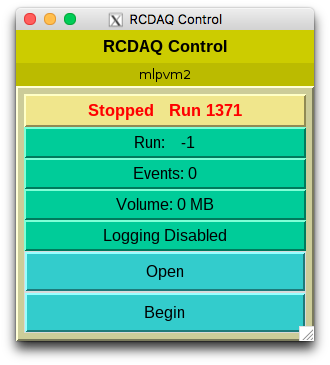
\includegraphics[height=2in]{rcdaqcontrol_idle.png} & 
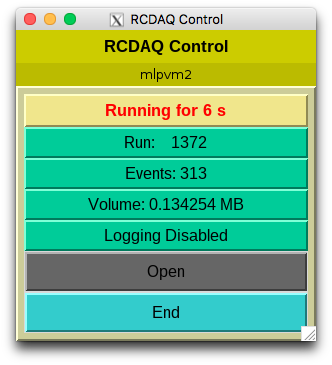
\includegraphics[height=2in]{rcdaqcontrol_no_logging.png}\\
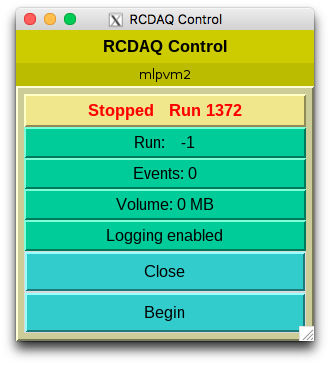
\includegraphics[height=2in]{rcdaqcontrol_loggingenabled.png} & 
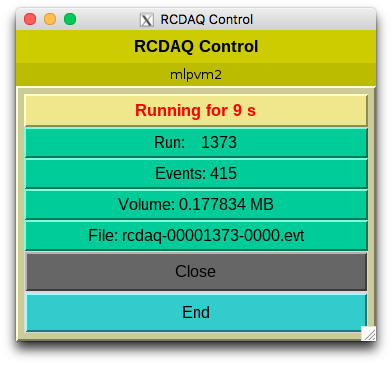
\includegraphics[height=2in]{rcdaqcontrol_logging.png}\\
\end{tabular}
\end{center}

\subsection{The Status GUI}

This GUI is essentially a stripped-down version of the control GUI. It
does not have the action buttons.  If you just want to keep an eye on
the status, there is no danger that you inadvertently click a button and 
interfere with the data taking. 

You start it with 

\begin{verbatim}
rcdaq_status.pl &
\end{verbatim}

and get 

\begin{center}
\label{rcdaqstatus}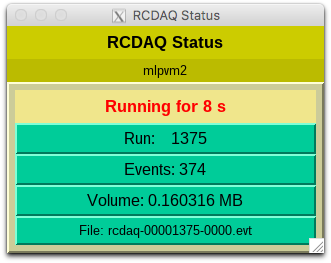
\includegraphics[height=2in]{rcdaqstatus.png}
\end{center}

Since this is a completely passive GUI, you can also use it to display
the status on an overhead monitor which is found in many control
rooms.  For that reason, it supports three options, \verb|--large|,
\verb|--display=<display>|, and \verb|--geometry=<geometry>|.  The
\verb|--large| option enlarges the GUI so that you can see it from a
distance, and the other options allow you to send it to a remote
display and position it properly, for example
 
\begin{verbatim}
rcdaq_status.pl --display=phnxtv1.phenix.bnl.gov:0.0 --geometry=+100+100 --large &
\end{verbatim}

\subsection{The Run Type Chooser GUI}

If you have run types defined, say, along the example from before

\begin{verbatim}
$ daq_list_runtypes
             beam - /data/rcdaq/beam/beam_%010d-%04d.evt
      calibration - /data/rcdaq/calibration/calibration_%010d-%04d.evt
             junk - /data/rcdaq/junk/junk_%010d-%04d.evt
         pedestal - /data/rcdaq/pedestal/pedestal_%010d-%04d.evt
\end{verbatim}

then you can easily select the type with this GUI. Type

\begin{verbatim}
rcdaq_runtypechooser.pl &
\end{verbatim}

and you will get 

\begin{center}
\includegraphics[height=2in]{rcdaqruntypechooser.png}
\end{center}

Each defined type brings up a button which allows you to  select the run type
easily.

Despite appearances, this GUI is stateless, too. The buttons merely
set the run type in the rcdaq\_server, but the display is updated not
from the button click but from information from the server, so the GUI
will reflect the changes if you change the run type from the command line.

This GUI will gracefully deal with a shutdown of the server, however,
it will get confused if you change the list of run types. I think this
is a small inconvenience, because the run types are usually pretty
static. If they do change, this GUI needs to be restarted. 

\subsection{The Configuration GUI}

This brings us to our last GUI, which is a bit more complex. We are
supporting setups where the researchers are used to selecting the
setup from a long scroll-down list of pre-made standard
configurations, depending on what the experiment of the day is. This
in itself is not so difficult, but soon you run into a complication
in defining what such a ``setup'' actually is.

You will likely find the area teeming with a number of shell or perl
scripts for different purposes, along with the top-level scripts which
define the various setups.  It is good practice to have those
individual setup scripts call more generic other scripts with the
proper parameters, in order to avoid a proliferation of ``flat''
all-in-one scripts. This immediately leads to the need to identify the
actual top-level scripts which are meant to be listed in that
GUI. Attempts to seclude those in a particular area only have, quite
predictably, not worked.

For this reason, we invented a scheme in which we identify those
``GUI-grade'' scripts by certain tags, which are comments in the
script.

If you look at the \verb|setup.sh| example script in the main rcdaq
source directory, you will see the following comments:

\begin{verbatim}
#! /bin/sh

# the following line identifies this script as one to be
# listed in the configuration GUI

# --RCDAQGUI

# lines starting with the "--SC" tag are short comments
# (can be only one, later ones override earlier ones)

# --SC Top Level setup script with a random device

# lines starting with the "--SC" tag are long comments

# --LC This setup script is part of the RCDAQ distribution.
# --LC It uses the random device (i.e. no particular hardware)
# --LC and can run on any machine to give RCDAQ a spin.
# --LC It can serve as a template to develop your own setups. 
\end{verbatim}

The \verb|--RCDAQGUI| tag identifies this script as one to be listed
in the GUI. Then there are ``short comments'', which act as tooltip
help (when you hover the mouse), and ``long comments'', which are
displayed once you select the GUI.

If you run 

\begin{verbatim}
rcdaq_configmenu.pl &
\end{verbatim}

in the directory where this \verb|setup.sh| script resides, you will see

\begin{center}
\includegraphics[height=2in]{rcdaqconfigmenu1.png}
\end{center}

(in this case there is only one such script, but all ``GUI-enabled'' scripts will be
shown but not any others. If you hover the mouse, you will see the tooltip with the 
``short comment'' (which can only be one line):

\begin{center}
\includegraphics[height=2in]{rcdaqconfigmenu2.png}
\end{center}

Selecting this then displays the longer help text, and you can see if
this script is what you wanted:

\begin{center}
\includegraphics[height=2in]{rcdaqconfigmenu3.png}
\end{center}

Once selected, you can then choose to execute the script, or cancel. 

\section{Web-based Controls}
\label{webcontrols}

The GUIs shown in the previous chapter are based on the ``Tk''
graphics widget set and are implemented in Perl. While extremely
versatile, Perl-Tk is not readily available on every platform, and
requires additional libraries to be installed. On several Linux
flavors in widespread use, such as RedHat and Scientific Linux, Tk can
be installed but is not part of the software management system, and
needs to be installed from source. In addition, the Tk system requires
the availability of the X11 graphics system, which eliminates all
platforms that do no support X11, such as iPads and iPhones. On other
platforms like Windows and most smart phones and tablets, the ``Tk''
component is extremely difficult to install or is not available at
all.

Recent advances in web technologies have converted the web browser
into a viable platform for slow controls, with the advantage that the
underlying technologies are available in most modern browsers on
virtually any platform, including smart phones and tablets.

By adding a GUI technology that uses web-based controls, it is
possible to implement the RCDAQ GUIs in a truly platform-independent
fashion. This makes them available on platforms which could not
support the GUIs before, such as smart phones, tablets, and even
iPads, which have the most restrictive execution environment of all
platforms.


\subsection{The Web-based RCDAQ Control GUI}

\begin{figure}[htb]
  \begin{center}
    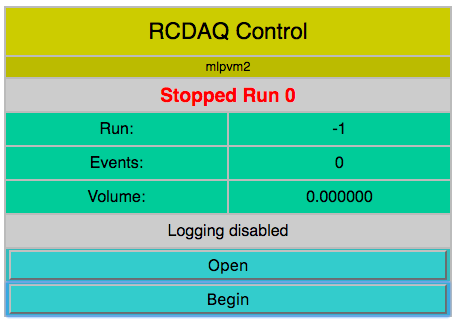
\includegraphics[width=0.47\columnwidth]{webcontrol_idle.png}
    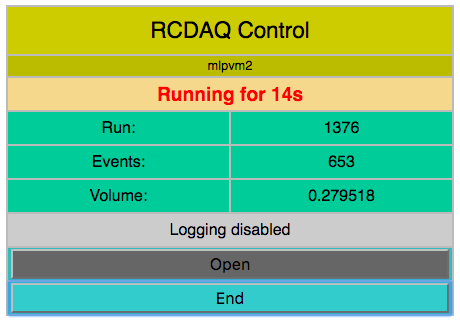
\includegraphics[width=0.47\columnwidth]{webcontrol_running.png}
    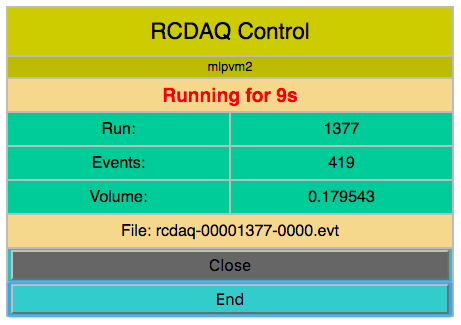
\includegraphics[width=0.47\columnwidth]{webcontrol_logging.png}
    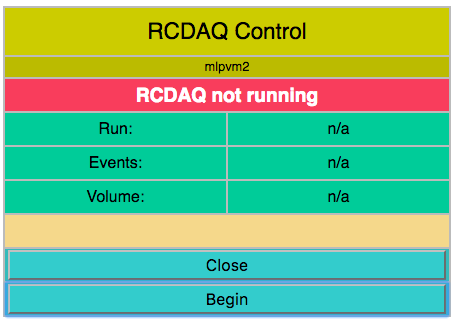
\includegraphics[width=0.47\columnwidth]{webcontrol_shutdown.png}
  \end{center}
  \caption{\label{webcontrol-idle}The new web-based control GUI for the RCDAQ system
    in various states of the RCDAQ operation. The upper left shows the GUI in the idle state, 
    then in the running state, while logging, and when the RCDAQ server has been shut down.}
\end{figure}

The web-based control interface acts like a web server running on the
chosen port. The default port is 8899, but you can choose any port
number that is available on your system.

The service starts automatically on port 8899. You can re-start it on a different port with the command
\begin{verbatim}
 rcdaq_client  daq_webcontrol <port number> 
\end{verbatim}

For example,
\begin{verbatim}
 rcdaq_client  daq_webcontrol
\end{verbatim}
starts the interface on the default port number 8899. You can then access the
web-based controls on your local machine where RCDAQ is running as
\begin{verbatim}
 http://localhost:8899
\end{verbatim}
or on another system as
\begin{verbatim}
 http://your.daq.machine:8899
\end{verbatim}

\warning{If you select another port number, keep in mind that RCDAQ is
  running without special privileges and cannot use any privileged
  ports such as the ``http'' port 80. If you use a port number
  different from the default, you \emph{must} use a non-privileged
  port higher than 1024, and it is recommended that you use a port
  number above 8000.}

At this point in time, only the equivalent of the standard control GUI
has been implemented as a web-based control. The web-based equivalent
of the ``Status'' GUI, shown on page~\pageref{rcdaqstatus}, will be
implemented in an upcoming version.

Over time, the web controls will make it easy to add other amenities
such as ready-made strip charts of the system performance, such as
``events taken per minute'' or ``data volume as a function of time''.

\begin{figure}[htb]
  \begin{center}
    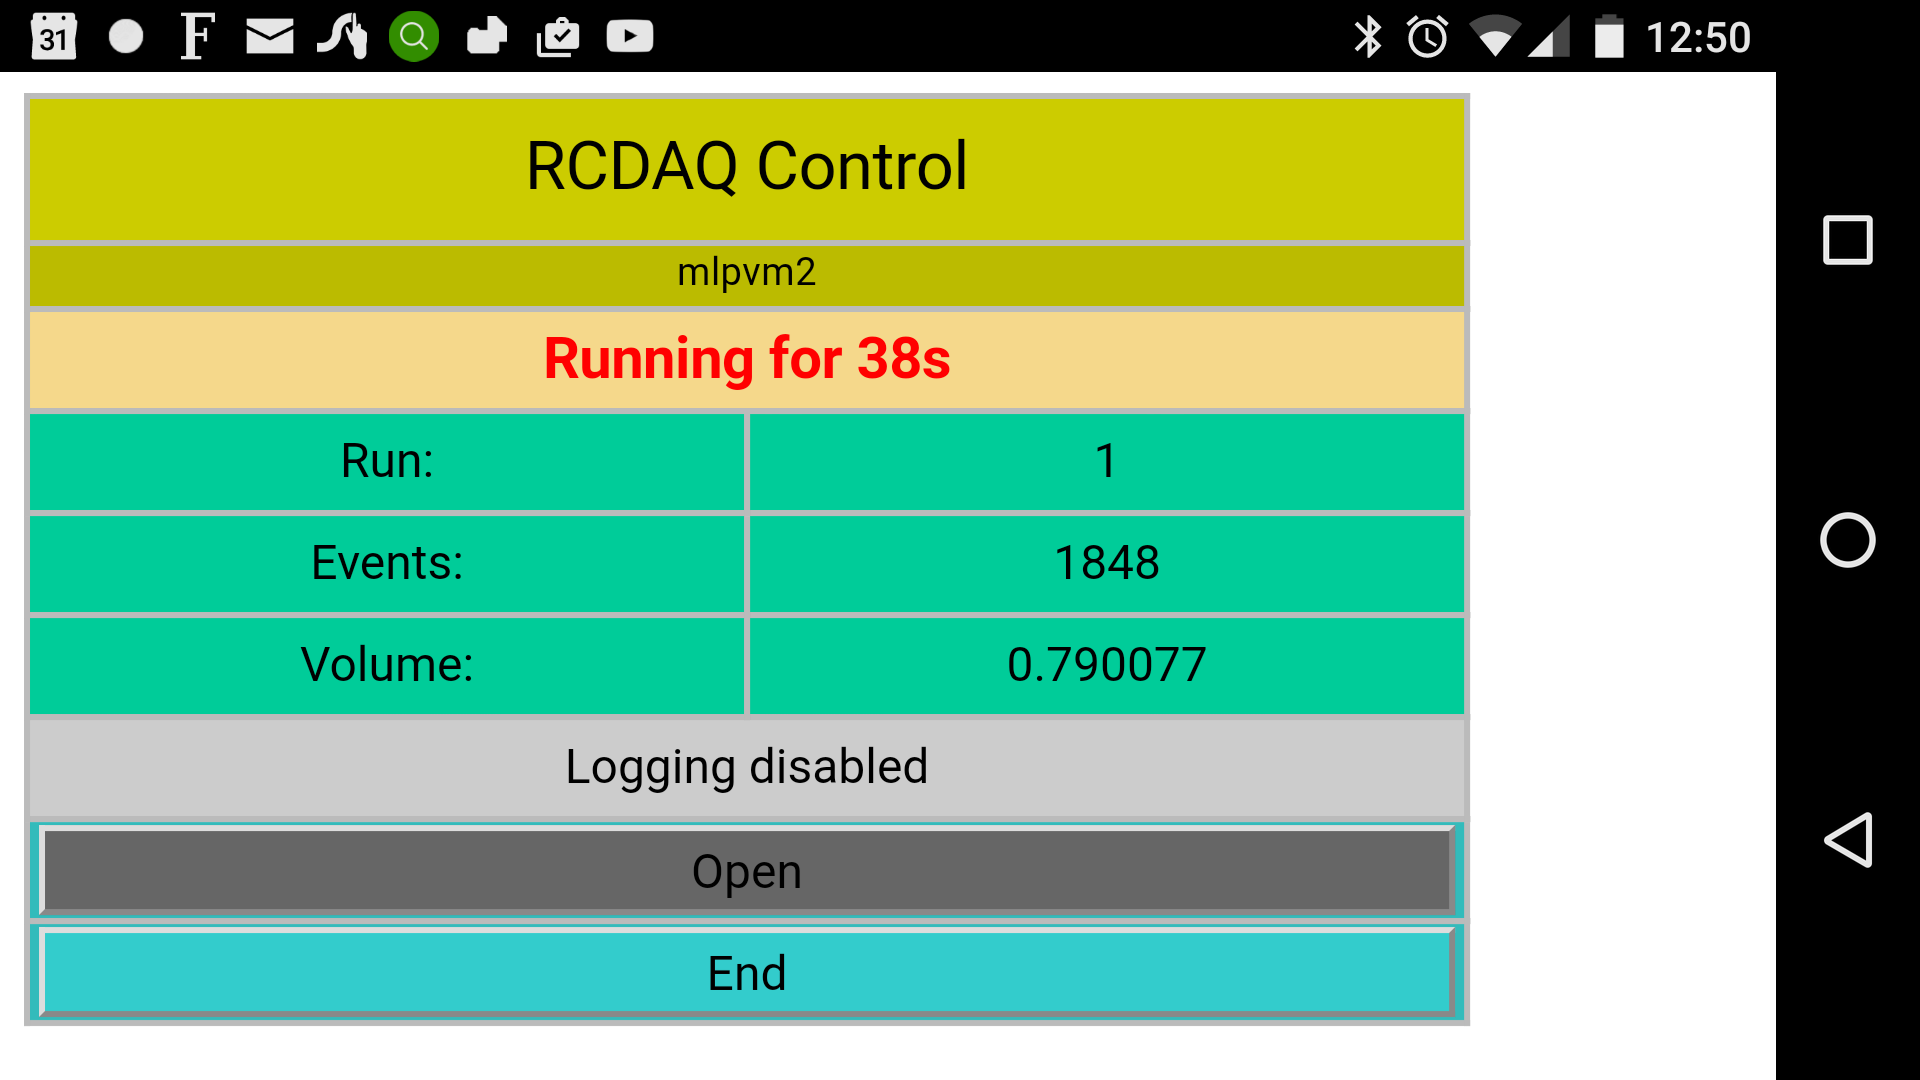
\includegraphics[width=0.85\columnwidth]{android.png} 
  \end{center}
  \caption{\label{android}The new web-based controls for the RCDAQ system
    running in the web browser on an Android phone.}
\end{figure}

To show the enhanced possibilities of the web-based controls,
Fig.~\ref{android} shows a screen shot of the controls running in the
browser on my Android phone. In the same way, it is now possible to
run the controls on iPads and basically any platform with a modern web
browser.


\section{Installation}
\label{installation}

If you want to give RCDAQ and the assorted analysis tools a quick look
(and potentially want my help at some point), it is easiest if you
follow these steps.

While there is nothing wrong with installing only the actual RCDAQ
component (and on a Raspberry Pi, it is rather difficult to go beyond
that), you typically want the analysis tools, too, in order to be able
to look at the data.

Obviously you can name your installation areas whatever you want, and
also install everything in the standard system areas. However, to get
started and make it easy for me to help you if needed, you might just
install it in the way I describe here so I can find my way around.

Especially the use of the environmental variable \verb|ONLINE_MAIN| is
convenient in the sense that it allows you to install all
sub-components (and later all plugins you wish to build) into the same
area easily. Still, if you are an expert user and proficient with the
UNIX auto-tools, nothing will prevent you from installing it in a way
that makes the most sense to you.

Here is how I recommend to begin:

Make a directory {\tt \$HOME/softwarerepo}, and ``cd'' there:

\begin{verbatim}
mkdir $HOME/softwarerepo
cd $HOME/softwarerepo
\end{verbatim}

git clone the rcdaq and online\_distribution components:

\begin{verbatim}
git clone https://github.com/sPHENIX-Collaboration/rcdaq.git
git clone https://github.com/sPHENIX-Collaboration/online_distribution.git
\end{verbatim}

Define an environmental variable \verb|ONLINE_MAIN|:

\begin{verbatim}
export ONLINE_MAIN=$HOME/softwarepo/install
\end{verbatim}

Generate the various build areas:

\begin{verbatim}
mkdir -p build/rcdaq
mkdir -p build/online_distribution/{eventlibraries,pmonitor}
\end{verbatim}

and move to respective area, configure, and install:

\begin{verbatim}
cd build/rcdaq
../../rcdaq/autogen.sh --prefix=$ONLINE_MAIN
make install|
\end{verbatim}

\begin{verbatim}
cd ../online_distribution/eventlibraries
../../../online_distribution/eventlibraries/autogen.sh --prefix=$ONLINE_MAIN
make install
\end{verbatim}

\begin{verbatim}
cd ../online_distribution/pmonitor
../../../online_distribution/pmonitor/autogen.sh --prefix=$ONLINE_MAIN
make install
\end{verbatim}


After the installation is complete, you should add the
\verb|$ONLINE_MAIN/bin| area to the \verb|PATH|, and define
\verb|$ONLINE_MAIN/lib| as \verb|LD_LIBRARY_PATH| (or add to an
existing definition).

You can then add the following lines to your
\verb|$HOME/.bash_login| or equivalent file for your shell:

\begin{verbatim}
export ONLINE_MAIN=$HOME/softwarerepo/install
PATH=$PATH:$ONLINE_MAIN/bin
export LD_LIBRARY_PATH=$ONLINE_MAIN/lib

source $ONLINE_MAIN/bin/aliases.sh

export ROOT_INCLUDE_PATH=$ONLINE_MAIN/include:$ONLINE_MAIN/include/Event:$ONLINE_MAIN/include/pmonitor
\end{verbatim}

The second-last line sets up the aliases as described in
chapter~\ref{convenience}. The last line is required if you are using
ROOT version 6 for your analysis. It defines where ROOT is looking for
the include files.



\section{System Requirements}

RCDAQ runs without special privileges. The only system service it
needs is \verb|rpcbind|, which typically gets started at boot time of
your system. The only modification to the usual way the rpcbind
service is run is that it \emph{may} need the ``-i'' flag. Test first
if all works without it before you change anything.

The end result must be that rpcbind is running, as shown here with the
``-i'' flag:

\begin{verbatim} 
$ ps ax | grep rpcbind
 2273 ?        Ss     0:00 /sbin/rpcbind -i
 5626 pts/0    S+     0:00 grep --colour=auto rpcbind
$
\end{verbatim}

Should you system require the -i flag, the way that is accomplished varies
a lot between Linux distributions. Here are a few of the more
mainstream ones:

\begin{description}

\item[Gentoo]  Create or edit the file \verb|/etc/conf.d/rpcbind|. Add a line

\begin{verbatim} 
RPCBIND_OPTS="-i"  
\end{verbatim}

\item[Scientific Linux]  Create or edit the file \verb|/etc/sysconfig/rpcbind|. Add a line

\begin{verbatim} 
RPCBIND_ARGS="-i"  
\end{verbatim}

\item[Ubuntu]  Create or edit the file \verb|/etc/default/rpcbind|. Add a line

\begin{verbatim} 
OPTIONS="-i"  
\end{verbatim}

\end{description}



\appendix

\section{Examples}

I show a few examples of real-life setups that were used in the past.

I will expand on this chapter as time progresses.

\subsection{Running Speed Tests}
\label{speedtests}
Let's say that you want to see how fast your system can take data when
you pull out all the stops. Actually reading out devices later will
invariably slow you down, but it is good to know where the limits of
your disk, CPU, and network are.

I mentioned the \verb|daq_device_deadtime| pseudo-device. It may sound
odd that you can use a device that adds artificial deadtime for a
speed test, but here is how it works.

Let me first show how to actually generate artificial deadtime. At the
time I write this at the FermiLab Test Beam Facility, it is unclear if
we will need this for the benefit of a MWPC, which may be able run at
only 100Hz (remains to be seen). Then we would add, say, 150 microseconds
deadtime:

\begin{verbatim}
rcdaq_client create_device device_deadtime 1 0 150
\end{verbatim}

The 3rd parameter is the deadtime added in units of the Unix \verb|usleep|
system call, which is meant to be microseconds, but you may have to calibrate and 
adjust the unit on your system a little bit.  

With the above parameters, it will not add anything to the data stream
(that's why the packet id is set to 0). It can, however, add an
adjustable amount of data to the event (and generate a packet,
obviously). And it can also provide the system trigger. That allows
you to dial in any desired data rate. Here is how you run the speed
test: You set the deadtime to 0 (no deadtime), set a packet id (I
chose 1005 here), have the device add 64 (32-bit) words to the event,
and provide the system trigger (the last ``1''). Since this is now the
only device defined in a data event, it will run as fast as it can:

\begin{verbatim}
rcdaq_client create_device device_deadtime 1 1005 0 64 1
\end{verbatim}

You can reduce the number of words to test the inner mechanics of
RCDAQ on your PC (how fast it can go through the paces to kick off the
event reading), or increase the number to test the limits of your
storage system. 

Be warned, though, that the artificial data do not have meaningful
values. Different from the \verb|device_random|, this device wastes
no time filling in any actual values; it just says that it has added
so many words, no matter what the contents of the packet payload are.

\subsection{Measuring Event Timing}
\label{eventtiming}

Especially under test beam conditions, it is often useful to see what
the ``spacing'' in time between events is. Ideally, you would expect a
somewhat balanced distribution with events being apart in time by
roughly the same amount, but very often you find that there is a
macroscopic structure in that distribution for a myriad of reasons.

If you see that in a beam setting, you should definitely find out why
that is. This usually points to some undesired feature in the beam,
which might have a microstructure, or some other structure. 

A trivial way of getting such an artificial structure is to have a
really slow file system to write the data to, such as a USB stick or
something similarly slow. Then the time it takes to write out a buffer to
storage is much longer than the time it takes to fill it. RCDAQ uses a
double-buffering scheme so one buffer is getting filled while 
another one is being written to disk. In modern solid-state disks and
especially in today's RAID systems, the writing is virtually always
faster than the filling. However, if the writing is slow, the readout
needs to wait for the writing to complete before that buffer becomes
available again, and the busy goes up.

In order to measure the distance between events, the system offers a
built-in pseudo device \verb|device_rtclock|. This device uses the
\verb|clock_gettime| system service and retrieves the
\verb|CLOCK_MONOTONIC_RAW| system clock, which is strictly continuous
and not affected by ``jumps'' due to NTP-driven or manual time
adjustments. The clock reports clock ticks in units of nanoseconds,
but that may need a system-dependent calibration. Still, it provides a
``heartbeat'' to gauge the relative timing of events. 

The device records both the current clock value, as well as the same
value from the last event where the ``device'' was read out. This
makes it easy to compute the relative timing of events.

Here is an example how to set up such a pseude device in a data event:

\begin{verbatim}
rcdaq_client create_device device_deadtime 1 1010
\end{verbatim}

It does not take any configuration parameters, only the event type and
the packet id.

\subsection{Adding a webcam picture to a packet}

In this setup we use a detector that gets positioned with a step
motor. While we save the motor positions in the begin-run event, it is
nice to have a visual confirmation that the detector is in the right
place, or actually moves in the direction we expect it to. To get
this, we add a webcam picture to the begin-run event. The webcam looks
at the detector with a ruler in the background, so you get a rough
verification that the detector at least moves in the right direction.

While there are many ways to get a webcam picture, the most flexible
solution is to run the ``\verb|motion|'' utility on the
system. \verb|motion| is a surveillance tool designed to monitor a
video stream and record video whenever \emph{motion} is detected in
the feed, where motion can be defined in a highly flexible manner. In
addition, the utility provides a web interface to a live video stream,
and has the ability to take snapshots in predefined intervals
independent of detected motion in the picture. All streams and
pictures carry a time stamp.

I usually adjust the threshold for motion recognition rather high so
no actual video gets recorded, although that of course depends on your
setup. The sequence of snapshot files later provides a rough
timeline of events if needed. The web interface allows you to remotely
monitor the camera at any time. For getting a picture from the camera,
I provide a simple perl script in the distribution which reads the web
live stream and extracts and saves one frame.

The script is called ``\verb|motion_cam_parse.pl|'' and takes the URL
of the webcam feed as an argument. Assuming that motion runs on the
local machine and the live feed appears on the standard port 8081, we can
get one picture:

\begin{verbatim}
motion_cam_parse.pl http://localhost:8081 > cam_picture.jpg
\end{verbatim}

I usually wrap this into a shell script ``\verb|capture_picture.sh|'':

\begin{verbatim}
#! /bin/sh
# this captures a picture to the provided filename,
# or cam_picture.jpg

FILE="$1"
[ -z "$FILE" ] && FILE=cam_picture.jpg
motion_cam_parse.pl > "$FILE"

\end{verbatim}

and then we configure rcdaq as follows:
\label{packet900}

\begin{verbatim} 
#! /bin/sh

D=`dirname "$0"`
B=`basename "$0"`
MYSELF="`cd \"$D\" 2>/dev/null && pwd || echo \"$D\"`/$B"
rcdaq_client create_device device_file 9 900 "$MYSELF"

# add the camera picture
rcdaq_client create_device device_command 9 0 "/home/eic/capture_picture.sh /home/eic/cam_picture.jpg"
rcdaq_client create_device device_file_delete 9 940 /home/eic/cam_picture.jpg

# .. lines deleted...
\end{verbatim}

We use \verb|device_file_delete| so it is impossible to add a stale
picture if there is a problem getting the current one.

\subsection{The GEM Detector Readout at the FermiLab Test Beam, February 2014}

This setup is building on the previous example in the sense that 
we are adding a lot of configuration information and two camera 
snapshots to the begin-run event. We also have 5 different run types defined.

First, we let the main RCDAQ configuration script figure out if there
is a \verb|rcdaq_server| running by issuing a \verb|daq_status|
command and testing its return status. If that fails, we need to start
the server. At this point, we also define the Elog whereabouts.

\begin{verbatim} 
#! /bin/sh

if ! rcdaq_client daq_status > /dev/null 2>&1 ; then
    echo "No rcdaq_server running, starting..."
    rcdaq_server > $HOME/log/rcdaq.log 2>&1 &
    sleep 2
    ELOG=$(which elog 2>/dev/null)
    [ -n "$ELOG" ]  && rcdaq_client elog localhost 666 RCDAQLog
fi
\end{verbatim} 

This is the ``make an absolute path'' routine you already know:

\begin{verbatim} 
# we need the $0 as absolute path b/c we pass it on to a "file" device further down
D=`dirname "$0"`
B=`basename "$0"`
MYSELF="`cd \"$D\" 2>/dev/null && pwd || echo \"$D\"`/$B"
\end{verbatim} 

We make the current run number persistent:

\begin{verbatim} 
rcdaq_client daq_setrunnumberfile $HOME/.last_rcdaq_runnumber.txt
\end{verbatim} 

And we find out if the SRS plugin is loaded already:

\begin{verbatim} 
if ! rcdaq_client daq_status -l | grep -q "SRS Plugin" ; then
    echo "SRS plugin not loaded yet, loading..."
    rcdaq_client load librcdaqplugin_srs.so
fi
\end{verbatim} 


And now we assemble the pieces that we want to add to the begin-run event. 
\begin{itemize}
\item Packet 900 will hold the configuration script itself
\item we execute the command \verb|srs_control readapv > $HOME/apv.txt|. It extracts 
most of the relevant setup parameters from the SRS crate and writes it to the file.
\item we execute  \verb|/home/eic/rcdaq_setup/prepare_run.sh|. This script 

\begin{itemize} 
\item reaches out to the motor rotation controller, queries the current
  position, and writes the value into \verb|current_position.txt|;
\item turns on a small light underneath the turntable for a moment and
 takes a picture from a webcam which looks at the scale for visual confirmation; the picture goes into an image file called
``\verb|snapshot.jpg|'';
\item it makes a similar snapshot from a permanently mounted overhead camera as ``\verb|overhead_snapshot.jpg|''.
\end{itemize}

\item we then add the ``\verb|apv.txt|'' file as packet 910;
\item we add ``\verb|current_position.txt|'' as packet 940; 
\item we add ``\verb|snapshot.jpg|'' as packet 941;
\item and we add ``\verb|overhead_snapshot.jpg|'' as packet 942.
\end{itemize}

\begin{verbatim} 
# we add this very file to the begin-run event
rcdaq_client create_device device_file 9 900 $MYSELF

rcdaq_client create_device device_command 9 0 "srs_control readapv > $HOME/apv.txt"
rcdaq_client create_device device_command 9 0 "/home/eic/rcdaq_setup/prepare_run.sh"

rcdaq_client create_device device_file 9 910  $HOME/apv.txt
rcdaq_client create_device device_file 9 940  $HOME/current_position.txt
rcdaq_client create_device device_file 9 941  $HOME/snapshot.jpg 128000
rcdaq_client create_device device_file 9 942  $HOME/overhead_snapshot.jpg 128000
\end{verbatim} 

The remainder of the set up script is straightforward; we set up the run types, 
set ``junk'' as default, and finally define the readout of the SRS crate:

\begin{verbatim} 
rcdaq_client daq_define_runtype beam    /data/gem/beam/beam_%010d-%04d.evt
rcdaq_client daq_define_runtype noSi    /data/gem/noSi/no_si_%010d-%04d.evt
rcdaq_client daq_define_runtype junk    /data/gem/junk/junk_%010d-%04d.evt
rcdaq_client daq_define_runtype calibration /data/gem/calibration/calibration_%010d-%04d.evt
rcdaq_client daq_define_runtype pedestal /data/gem/pedestal/pedestal_%010d-%04d.evt
rcdaq_client daq_setruntype junk

rcdaq_client create_device device_srs 1 1010 10.0.0.2 1
\end{verbatim} 
 
And here is the composition of the begin-run event:

\begin{verbatim} 
$ dlist -i -t 9 beam_0000000451-0000.evt
 -- Event     1 Run:   451 length: 17431 type:  9 (Begin Run Event)  1392306649
Packet   900   614 -1 (ONCS Packet)  4 (IDCSTR)
Packet   910   142 -1 (ONCS Packet)  4 (IDCSTR)
Packet   940     7 -1 (ONCS Packet)  4 (IDCSTR)
Packet   941  3643 -1 (ONCS Packet)  4 (IDCSTR)
Packet   942 13017 -1 (ONCS Packet)  4 (IDCSTR)
\end{verbatim} 

If we now want to find out the position of the turntable, we can have  a
look at packet 940:

\begin{verbatim} 
$ ddump -t 9 -p 940  /media/psf/Home/srs/GEM/beam/beam_0000000472-0000.evt
-0000020
$
\end{verbatim} 

( -20 is actually the ``zero'' position, 80 ticks mean one degree, the the zero marks are aligned at this value.)

Here is another run:

\begin{verbatim} 
$ ddump  -t 9 -p 940  /media/psf/Home/srs/GEM/beam/beam_0000000474-0000.evt
+0002380
$ 
\end{verbatim} 

which is at 2380 (+20) ticks (30 degrees).

In case there seems something wrong, one can extract the webcam snapshots:

\begin{verbatim} 
$ ddump  -t 9 -p 941 beam_0000000472-0000.evt > 472.jpg
$ ddump  -t 9 -p 942 beam_0000000472-0000.evt > 472_overhead.jpg
$ ddump  -t 9 -p 941 beam_0000000474-0000.evt > 474.jpg
$ ddump  -t 9 -p 942 beam_0000000474-0000.evt > 474_overhead.jpg
\end{verbatim} 

Here you can see these snapshots:

\includegraphics[height=2in]{472.jpg}
\includegraphics[height=2in]{474.jpg}

\includegraphics[height=2in]{472_overhead.jpg}
\includegraphics[height=2in]{474_overhead.jpg}

This is great for potential forensics and a visual conformation that the detector
was at the right position. 



\section{A Selection of Currently Implemented Readout Devices}

\subsection{The PSI DRS4 Evaluation Board}
\label{instructions}

The DRS4 chip is a switched capacitor array capable of sampling at a
speed of up to 5\,Gigasamples/s. This device supports sampling rates
of 0.7, 1, 2, and 5\,GS/s. 

The PSI DRS4 evaluation board is one of the workhorse systems in small
setups. It offers 4 waveform digitizing channels with sample rates of
up to 5GS/s. Since it is a USB-based device, it can be run on
virtually any Linux system without the need for special
interfaces. Fig.~\ref{drsevalboard} shows pictures of the board.

This is the only device implemented in RCDAQ so far that is capable of
being read out with a Raspberry Pi. The RCDAQ core will work on a Pi
just fine, but most of the other readout devices will not be
supported, because the required vendor-supplied libraries are usually
not available. The DRS4 evaluation board is the exception. I have
personally used the board with a Pi for a long-term cosmic calibration
measurement, where I didn't want to commit a more powerful PC to
acquire the data.

To start, you need to make sure that your system has all the libraries
needed to interface with the DRS4 evaluation board in the first
place. Follow the instructions on the PSI website what to install and
configure.  You should be able to run the \verb|drsosc|
``oscilloscope'' application, shown in Fig.~\ref{drsosc}, on your
system \emph{before} you start with RCDAQ.

\begin{figure}
  \centering
  \includegraphics[width=0.4\columnwidth]{drsfront.jpg}
  \includegraphics[width=0.4\columnwidth]{drsback.jpg}
  \caption{\label{drsevalboard}The PSI DRS4 Evaluation Board.}
\end{figure}

The installation of the plugin follows the recipe outlined in
chapter~\ref{installation} exactly. Go back to the place where you
already installed RCDAQ, in my example from above
\verb|$HOME/softwarerepo|. Then get the software:

\begin{verbatim}
git clone https://github.com/sPHENIX-Collaboration/drs4.git
\end{verbatim}

and you will have a new directory ``drs4''. Now go to your build area,
\verb|$HOME/softwarerepo/build| in the example, make a new directory ``drs4'',
and configure:

\begin{verbatim} 
$ mkdir drs4 
$ cd drs4 
$ ../../drs4/autogen.sh --prefix=$HOME/softwarerepo/install 
$ make install
\end{verbatim}

This will install \verb|librcdaqplugin_drs.so| in your
\verb|$ONLINE_MAIN/lib| area, which is the plugin that teaches RCDAQ how
to read the Evaluation Board.

This is the way how you install every other plugin as well, just
replace the name accordingly.

You can now load the plugin, and see the effect with the
\verb|daq_status -ll| command:

{\footnotesize 
\begin{verbatim}
$ rcdaq_client load librcdaqplugin_drs.so
$ daq_status -ll
Stopped
Logging enabled
have a trigger object
Filerule:     rcdaq-%08d-%04d.evt
Buffer Sizes:     32832 KB adaptive buffering: 15 s
Web control Port:  8899
Elog: not defined
 -- defined Run Types:  (none)
List of loaded Plugins:
 - DRS Plugin, provides -
 -     device_drs (evttype, subid, triggerchannel, triggerthreshold[mV], slope[n/p], delay[ns], 
                   speed, start_ch, nch, baseline[mV]) - DRS4 Eval Board
 -     device_drs_by_serialnumber (evttype, subid, serialnumber, triggerchannel, 
                   triggerthreshold[mV], slope[n/p], delay[ns], 
                   speed, start_ch, nch, baseline[mV]) - DRS4 Eval Board
\end{verbatim}
}

\begin{figure}
  \centering
  \includegraphics[width=0.95\columnwidth]{drsosc.png}
  \caption{\label{drsosc}A screenshot of the drsosc application. Make
    sure that you can sucessfully run this application before you
    start setting up RCDAQ.}
\end{figure}

The only slightly complicated setting is the \verb|triggerchannel|
parameter, which is a bit-mapped value. You will usually see some
value such as \verb|0x21| here. The 5 least significant bits denote
the 4 inputs and the external trigger as triggers for the board.

Keep in mind that there are two different triggers here -- one is
triggering the board itself, and the other is whether or not this
board also provides the system trigger for RCDAQ (see
chapter~\ref{running} for the explanation). So bits 0-4 switch on or
off the 5 possible sources of board triggers, and bit 5 says if this
board generates the system trigger. So \verb|0x21| -- bits 0 and 5 are
set -- is saying that channel 1 triggers the board, and the board also
makes the system trigger. \verb|0x30| means the system trigger, and
the external trigger triggers the board. Keep in mind that if you
choose to \emph{not} make the system trigger here, you need another
device to do that; you will not get any events else.

There is another specialty in the standard Linux parameter
parsing that you need to think of and which is shown in this setup
example:

\begin{verbatim}
rcdaq_client create_device device_drs -- 1 1001 0x21 -150 negative 438 2
\end{verbatim}

Since we need to prevent the parser from interpreting the \verb|-150|
as options ( -1, -5, -0), you need to tell it to stop the option
parsing with the the ``double-dash'' -- \verb|--|. This is standard
Unix shell behavior, but you need to remember that.

The above line sets the board up to trigger on channel 1, negative trigger
with a -150\,mV threshold, an internal delay of 438 ticks (that's how
far we ``look back'' in the waveform before the trigger), and 2GS/s
speed. The final ``2'' parameter happens to mean 2GS/s, but this
parameter is enumerated:

\begin{center}
\begin{tabular}{|c|c|}
\hline
parameter & speed \\
\hline
\hline
    0 & 700\,MS/s  \\ \hline
    1 & 1\,GS/s   \\ \hline
    2 & 2\,GS/s   \\ \hline
    3 & 5\,GS/s   \\ \hline
\end{tabular}
\end{center}

By the way: The way I derive the delay and speed parameters is to run
\verb|drsosc|, adjust everything the way I want it, and then
transcribe the parameters from \verb|drsosc| to the setup command. If
you look at Fig.~\ref{drsosc}, you will see that I used the same
settings (2\,GS/s and a delay of 438 ticks) in the setup example
above.

There are two more ``hidden'' parameters which assume default values
when omitted.  The above setup command is equivalent to

\begin{verbatim}
rcdaq_client create_device device_drs -- 1 1001 0x21 -150 negative 438 2 0 1024
\end{verbatim}

where the last two parameters mean ``start channel'' and ``number of
samples''. Setting the former to a non-zero value will cut out the
early part of the waveform. I \emph{strongly} advise against using
this parameter, since this will actually slow down your system as it
involves copying the desired part of the waveform to the right place.
You can virtually always accomplish the same by adjusting the delay
value (or delaying the hardware trigger). It is here more
out of a sense of completeness.

With the ``number of samples'' parameter you can cut out the later
part of the waveform. For example, if your signal is confined to the
first 250 samples in your waveform, you can store just those first 250
samples. This will only save storage space and not gain any
significant readout speed, since we still need to read the full
waveform and only discard the unwanted tail end. Different from
discarding the front part, the tail end can be discarded without an
expensive copy operation.


\subsection{The CAEN DRS4 1742V System}


The CAEN V1742 module, shown in Fig.~\ref{caen1742v}, is one of the
more complex modules implemented in RCDAQ. At its core, it has 4 DRS4
chips inside, providing 32 primary input channels, plus one ``side''
channel per chip. Two of those can be used to digitize the NIM input
signal if so desired.

Different from the evaluation board, it supports sampling speeds of 1,
2.5, and 5\,GS/s.


The assorted RCDAQ plugin, \verb|librcdaqplugin_CAENdrs.so|, provides
two different devices to readout the V1742. One, called
\verb|device_CAENdrs|, uses the preconfigured V1742 as-is, without
changing any ``non-essential'' registers. This device makes the full
configuration space available that the V1742 has to offer. It comes
with a companion utility \verb|caen_client|, which can be used to
adjust any available register as needed. I said ``non-essential''
registers, because RCDAQ still sets up the registers that govern the
actual readout the way it needs it; there is not much choice in that
matter. Still, in this way one can set up any conceivable trigger
mode, readout length, sample, rate, and so on, essentially any
configuration parameter. Here is a list of parameters that the
\verb|caen_client| utility can set and read:

\begin{figure}
  \centering
  \includegraphics[angle=90,width=0.8\columnwidth]{1742v.jpg}
  \caption{\label{caen1742v}The CAEN V1742 module.}
\end{figure}


\begin{verbatim}
$ caen_client status
MaxNumEventsBLT:       1
ExtTriggerInputMode:   3 (ACQ_AND_EXTOUT)
FastTriggerDigitizing: 0 (Disabled)
FastTriggerMode:       0 (Disabled)
OutputSignalMode:      0 (TRIGGER)
Sampling Frequency:    2 (DRS4_1GHz)
RecordLength:          1024 samples
PostTriggerSize:       0
IOLevel()              0 (NIM)
AcquisitionMode        0 (software controlled)
GroupEnableMask        0xf
TriggerPolarity (F - falling edge / R - rising edge) :
  R  R  R  R  R  R  R  R
  R  R  R  R  R  R  R  R
  R  R  R  R  R  R  R  R
  R  R  R  R  R  R  R  R

ChannelDCOffset:
  0x8f00  0x8f00  0x8f00  0x8f00  0x8f00  0x8f00  0x8f00  0x8f00
  0x8f00  0x8f00  0x8f00  0x8f00  0x8f00  0x8f00  0x8f00  0x8f00
  0x8f00  0x8f00  0x8f00  0x8f00  0x8f00  0x8f00  0x8f00  0x8f00
  0x8f00  0x8f00  0x8f00  0x8f00  0x8f00  0x8f00  0x8f00  0x8f00
\end{verbatim}

This pretty much covers the entire configuration space of the device.

The other device you can define is \verb|device_CAENdrs_std|, which is
a no-frills standard configuration. It can also be adjusted by using
\verb|device_CAENdrs| and \verb|caen_client|, but for a novice user it
provides a guaranted-to-work way to configure the device. This device
will not obey the \verb|caen_client| changes but re-set everything to
its defaults at each begin-run. It takes a NIM signal on the
trigger line, and adjusts the offsets to a range of $\pm 500$\,mV.

The syntax is 

\begin{verbatim}
device_CAENdrs_std evttype  subid  trigger  speed  delay
\end{verbatim}

where "trigger" means whether or not the device provides the system trigger. 



\end{document}


